%\begin{savequote}[8cm]
%A process cannot be understood by stopping it. Understanding must move with the flow of the process, must join it and flow %with it. (First Law of Mentat)
%  \qauthor{--- Frank Herbert, Dune}
%\end{savequote}
%Edsger W. Dijkstra, How do we tell truths that might hurt? (1975).

\chapter{An introduction to design and simulation tools}
\label{ch:oxview_intro}

\minitoc

While previous chapters have covered modular self-assembly on a very abstract level, approximating the modules as simple cubes or patchy particles, this chapter will introduce tools and methods for designing and simulating individual structures or modules folded using DNA (or RNA).

The following sections will cover a selection of practical design and simulation tools that have been developed over the years, providing context for the presentation of my contributions to the \emph{oxView} tool in Chapter~\ref{ch:oxview}.

% REFER TO THIS OVERVIEW!! https://pubmed.ncbi.nlm.nih.gov/33920889/


%Simulating the structure and dynamics of individual DNA origami modules has been possible for a while, but my aim with this project has been to make such simulations more accessible and easy to use and analyse.

%This is accomplished as I develop new tools and scripts while learning about the simulation methods and the designs that various laboratories are interested in.

%This chapter describes the currently available tools for simulation and design of individual module structures. DNA and RNA structures can be digitally represented in many different formats, for many different uses, and with different levels of coarse-graining. 

%The following sections cover my results over the last year, investigating methods for converting designs into the oxDNA/RNA format and for visualising and analysing the simulation results.

\section{Design tools for DNA origami}\label{sec:design_tools}
Designing a DNA origami structure by hand would be very laborious for anything but the most simple design. As such, a host of computer-aided design tools have been introduced over the years to make things easier. This section will cover some of the more common examples.

\subsection{Lattice-based design tools}
The caDNAno design tool \cite{cadnano} and the web-based scadnano \cite{scadnano} it inspired, allows the user to design DNA origami structures on a lattice of parallel helices.

\subsubsection{caDNAno}
\label{sec:cadnano}
CaDNAno \cite{cadnano} was introduced in 2009 as a way to simplify 2D and 3D DNA origami design. It has a graphical user interface with multiple panels, as seen in Figure~\ref{fig:cadnano}. In the slice panel, the designer can place virtual helices on a lattice (either hexagonal or square), seen in the leftmost panel of the figure. The helices can then be filled in with strands and connected using crossovers in a path panel, seen in the middle of the figure.

Finally, caDNAno is also available as a plugin to the Autodesk Maya software, which enables a 3D visualisation of the design as seen in the render panel to the right in Figure~\ref{fig:cadnano}. However, caDNAno does not support Maya versions after 2015 \cite{cadnanoInstall}.

\begin{figure}[h]
  \begin{center}
    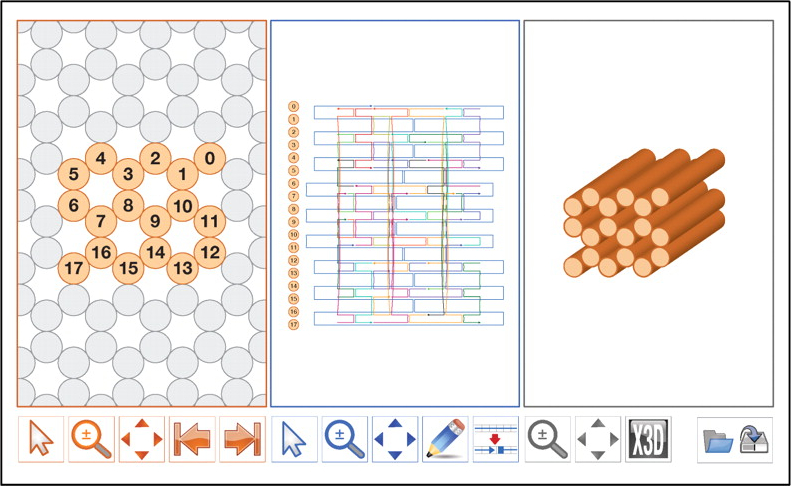
\includegraphics[width=\textwidth]{figures/cadnano.jpeg}
    \caption{The caDNAno design interface, adapted from \cite{cadnano}. The slice panel (left) shows helices as circles on a lattice, while the path panel (centre) shows individual strands from a flatened side view of the helices. The rightmost panel shows a 3D visualisation of the design.}
    \label{fig:cadnano}
  \end{center}
\end{figure}

\subsubsection{Scadnano}
Scadnano \cite{scadnano} (short for \emph{scriptable caDNAno}) is a relatively new design tool, independent from but inspired by caDNAno version 2. The main difference is that Scadnano is entirely web-based (thus not requiring any installation). The python code base is also designed to make it easier to write scripts generating DNA designs. Scadnano can be found at \url{https://scadnano.org/}.

\subsection{Top-down shape converters}
While tools like caDNAno simplify bottoms-up design, where the user builds structures from individual strands and nucleotides, a top-down tool can take a polyhedral target shape as input and provide a suitable origami design as output. 

% Mention DNA bricks software?

\subsubsection{BSCOR}
\label{sec:bscor}
%https://doi.org/10.1038/nature14586

In 2015, Benson et al. published a method for converting arbitrary mesh designs into a DNA origami mesh \cite{vHelix}. Figure~\ref{fig:bscor} shows a set of example polyhedral shapes, with the designed shape in Figure~\ref{fig:bscor}.a), the output DNA design in Figure~\ref{fig:bscor}.b), and microscopy characterisations in Figure~\ref{fig:bscor}.c-d). A follow-up paper in 2016 also introduced the ability to design flat-sheet meshes \cite{benson2016computer}. BSCOR uses single DNA duplex edges, with double edges added whenever topologically necessary.

\begin{figure}[h]
  \centering
  \begin{overpic}[width=\textwidth]{figures/bscor.png}
    \put(20,460){\small{1. Mesh generation}}
    \put(280,460){\small{2. Scaffold routing}}
    \put(520,460){\small{3. Spring relaxation}}
    \put(780,460){\small{4. Staple design}}
    \put(-30,550){a)}
    \put(-30,350){b)}
    \put(-30,210){c)}
    \put(-30,70){d)}
  \end{overpic}
  \caption{3D meshes rendered in DNA origami using BSCOR. Adapted from \cite{vHelix} and \cite{vHelixWeb}. \textbf{a)} Automated design process, where a scaffold is routed onto a mesh, each helix is relaxed using spring forces, and staple strands are added. \textbf{b)} Examples of initial meshes. \textbf{b)} Completed DNA designs with strands rendered as tubes. \textbf{c)} Negative-stain dry-state TEM micrographs of each design.}
  \label{fig:bscor}
\end{figure}


\subsubsection{ATHENA}
% DAEDAULS/PERDIX
%https://www.science.org/doi/full/10.1126/science.aaf4388
 %ATHENA? https://academic.oup.com/nar/advance-article/doi/10.1093/nar/gkab762/6368527 - Use fig 2 in now published paper!!!

 ATHENA is a recently published tool bundle for automatic designing wireframe origami shapes. As seen in Figure~\ref{fig:athena}, ATHENA brings together earlier software such as PERDIX, METIS, DAEDALUS and TALOS, into a single package capable of facilitating the design of both 2D and 3D wireframes with different edge designs.


\begin{figure}[h]
  \begin{center}
    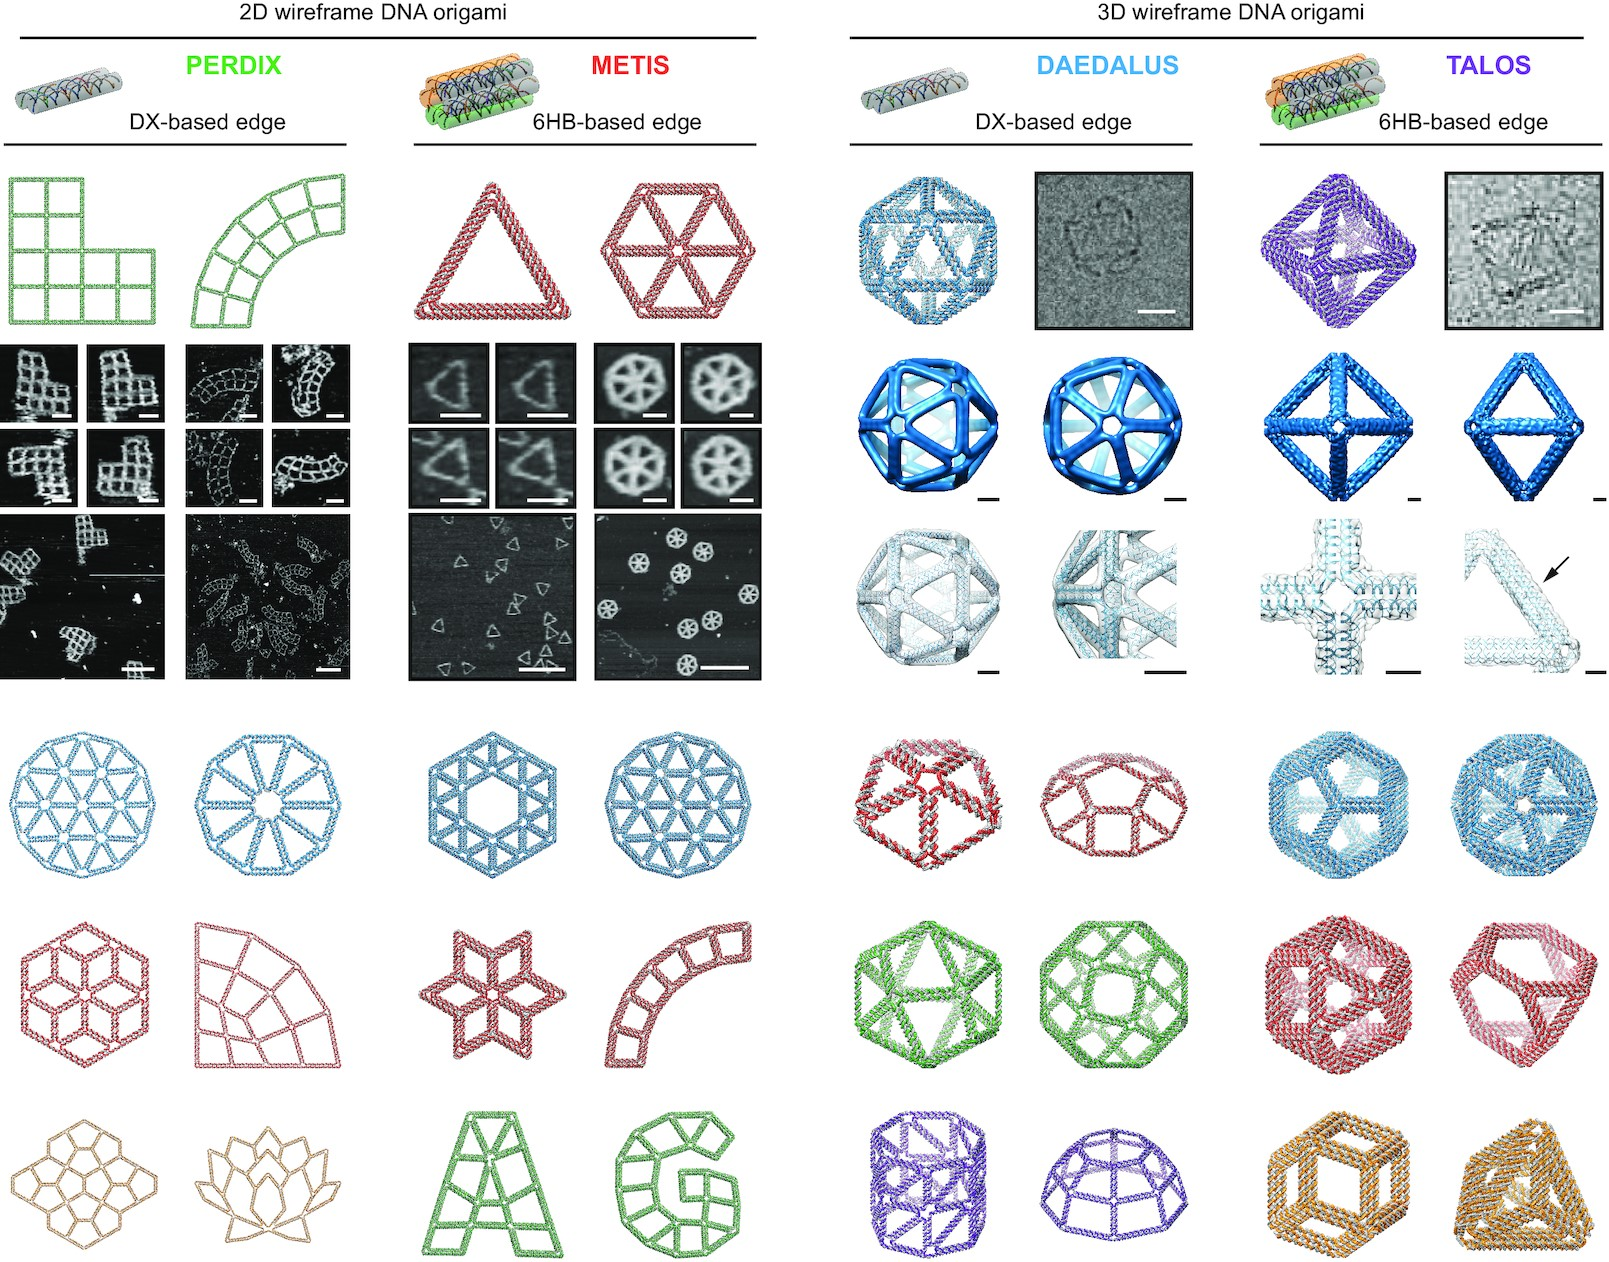
\includegraphics[width=\textwidth]{figures/athena.jpeg}
    \caption{Automatic wireframe origami shapes using ATHENA. Adapted from \cite{athena}. ATHENA includes the previous design packages PERDIX, METIS DAEDALUS and TALOS for 2D and 3D wireframe design, using double crossover (DX) and six-helix bundle (6HB) edges respectively. }
    \label{fig:athena}
  \end{center}
\end{figure}

%\subsubsection{Triangulated truss structures}
% M. Matthies
% https://pubs.acs.org/doi/abs/10.1021/acs.nanolett.6b00381

\subsection{Free-form or hybrid tools}
The final category of design tools is either free-form, where designs are drawn without a lattice, or hybrid tools combining both lattice and free-form design. 

\subsubsection{Tiamat}
\label{sec:tiamat}
Tiamat is an early free-form design tool (introduced in 2009) \cite{Tiamat} running exclusively on Microsoft Windows. The second version of can handle both DNA and RNA designs, either drawing them from scratch or importing them from PDB files. It can also export JSON format for easier conversion to other formats. See Figure~\ref{fig:tiamat} for a screenshot of the user interface of Tiamat 2, where a DNA tetrahedron is loaded.

\begin{figure}[h]
  \begin{center}
    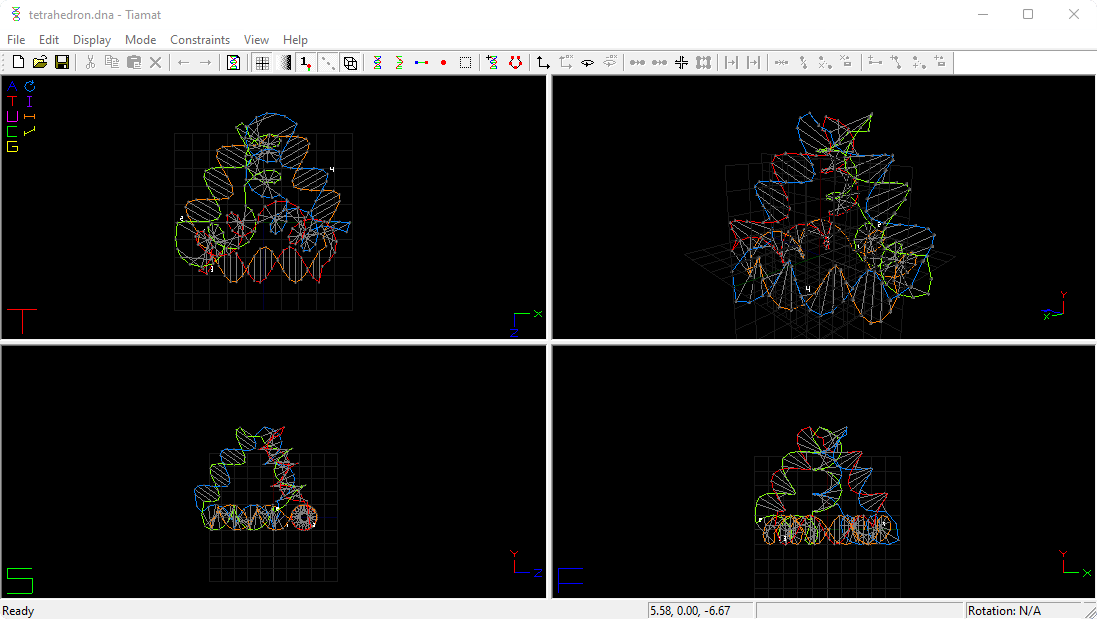
\includegraphics[width=\textwidth]{figures/tiamat_ui.png}
    \caption{A screenshot of the Tiamat \cite{Tiamat} (v2) user interface. The loaded tetrahedron design is from the Yan Lab resources page \cite{tiamatWeb}}
    \label{fig:tiamat}
  \end{center}
\end{figure}

\subsubsection{vHelix}
\label{sec:vhelix}
The free-form tool vHelix \cite{vHelix} is a plugin for the commersial Autodesk Maya software and was developed together with the BSCOR toolkit. Users can import the ``rpoly'' wireframe result from BSCOR, create designs from scratch, or import caDNAno files. It is also possible to export oxDNA simulation files. An example of the vHelix interface is shown in Figure~\ref{fig:vhelix}. 

\begin{figure}[h]
  \begin{center}
    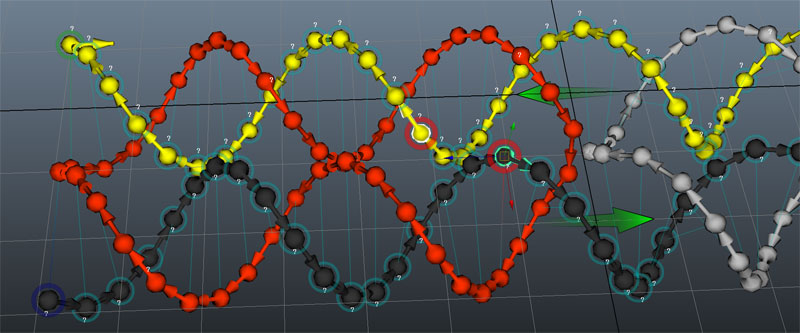
\includegraphics[width=\textwidth]{figures/vhelix.jpg}
    \caption{Free-form editing in vHelix. Image is from the vHelix website \url{http://www.vhelix.net/} \cite{vHelixWeb}.}
    \label{fig:vhelix}
  \end{center}
\end{figure}


\subsubsection{Adenita}
Adenita \cite{miao_tvcg_2018} is a hybrid free-form editing tool developed as a plugin to the commersial SAMSON toolkit. As seen in Figure~\ref{fig:adenita}.a), the design can be visualised and edited at multiple levels of abstraction, from an all-atom representation, through nucleotides and strands to cylinders representing entire helices. Strands can be drawn on a lattice in a 2D view, or edited in 3D. Figure~\ref{fig:adenita}.b) shows some of the available editing and visualisation tools. Note, for example, the wireframe creation tool based on the Daedalus algorithm. Adenita can also load caDNAno files and export oxDNA simulation files.

Like vHelix (Section~\ref{sec:vhelix}), Adenita is tied to the editor it is a plugin to, requiring the user to install both.


\begin{figure}[h]
  \begin{center}
    \begin{overpic}[width=\textwidth]{figures/adenita.jpg}
      \put(-20,400){a)}
      \put(-20,100){b)}
    \end{overpic}
    \caption{Adenita, adapted from \cite{miao_tvcg_2018}. \textbf{a)} A DNA double-helix visualised at different abstraction levels, with a purple band highlihghting a specific base-pair at all the four main levels. \textbf{b)} Available editing and visualisation tools in Adenita.}
    \label{fig:adenita}
  \end{center}
\end{figure}

\subsubsection{MagicDNA}
MagicDNA \cite{huang2021integrated} is another hybrid design tool using orientable lattices. As seen in Figure~\ref{fig:magicDNA}, it has a computer-aided design workflow where geometry can be specified from helix cross-sections or imported from a part library, then assembled and oriented into an integrated structure (using multiple scaffolds if necessary). MagicDNA is built as an application for the MATLAB software, so (like the previous two tools) installation requires a commersial third-party tool.


\begin{figure}[h]
  \begin{center}
    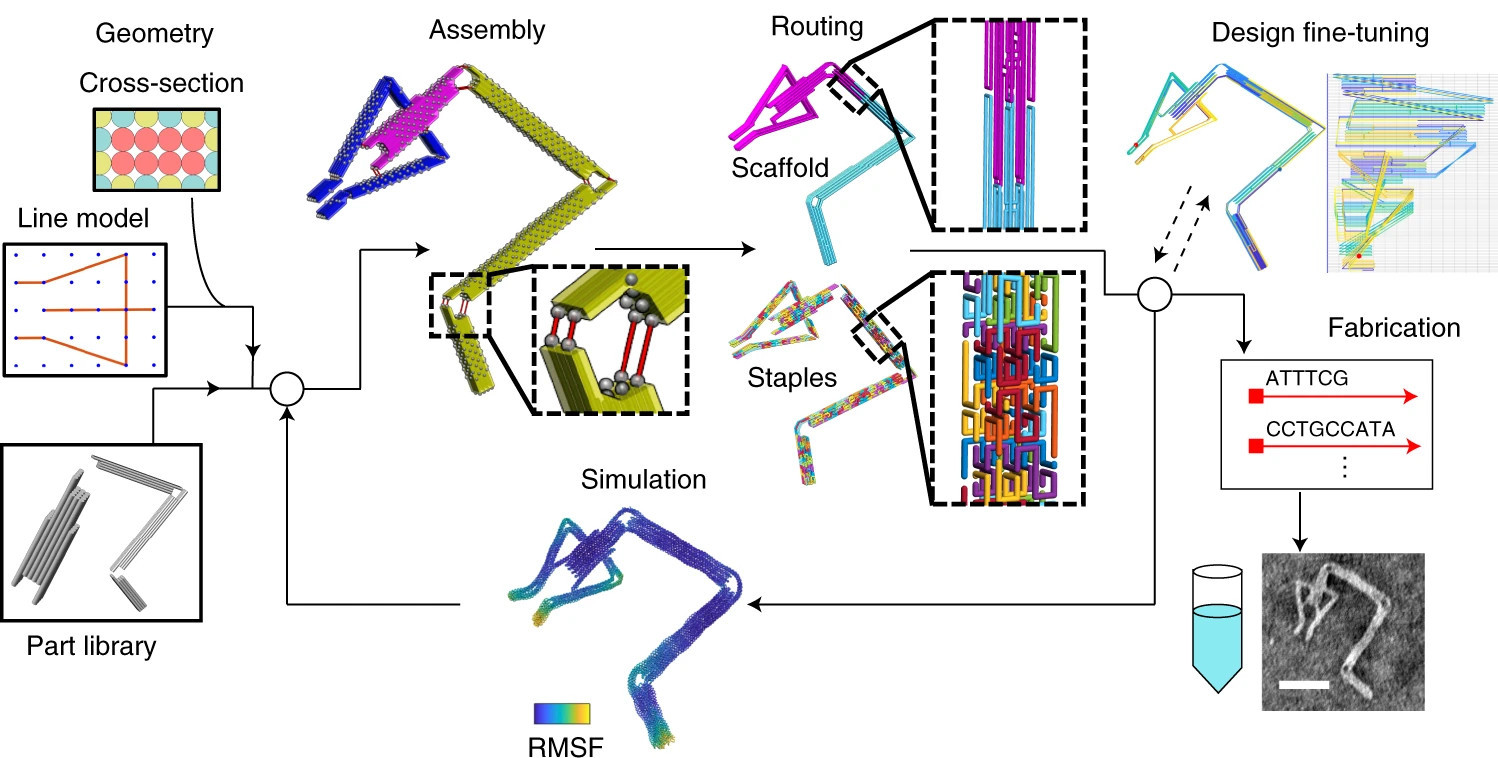
\includegraphics[width=\textwidth]{figures/magicDNA.jpeg}
    \caption{MagicDNA design workflow, adapted from \cite{huang2021integrated}. Assemblies can be created from line drawings and helix cross sections or imported from a library of parts. After strand routing and some optional fine-tuning in caDNAno, designs can be exported as sequences for fabrication or oxDNA files for simulation.}
    \label{fig:magicDNA}
  \end{center}
\end{figure}

\subsubsection{OxView}
The oxView application \cite{poppleton2020design, bohlin2021design} was developed as part of this thesis project and will be described more in Chapter~\ref{ch:oxview}. Compared to the other design tools introduced here, oxView aims to excel in combining designs from various formats, as well as easily preparing structures for oxDNA simulation (Section~\ref{sec:oxDNA}). Finally, oxView does not require any installation and is immediately available as a web-app at \url{www.oxview.org}.

\section{Nucleic acid simulation models}
Simulating a structure can both guide decisions at the design stage and provide insight for understanding experimental results. Coarse-grained models tend to run faster, but may lose some accuracy compared to models with more detail. This section covers simulation models at an increasing level of coarse-graining, from individual atoms to cylindrical helices.

\subsection{All-atom simulation}
Simulation tools such as NAMD \cite{NAMDphillips2005scalable}, use force fields such as AMBER \cite{AMBERcornell1996second} and CHARMM \cite{brooks1983charmm} to model interactions between individual atoms. While it is possible to perform atomistic simulations of large DNA origami structures \cite{yoo2013situ} as shown in Figure~\ref{fig:all-atom}, the simulations take a long time to run, and it is unknown how well the models represent DNA thermodynamics \cite{sengar2021primer}.

%Also cite Pointer origami https://academic.oup.com/nar/article/44/7/3013/2467847 ?

\begin{figure}[h]
  \begin{center}
    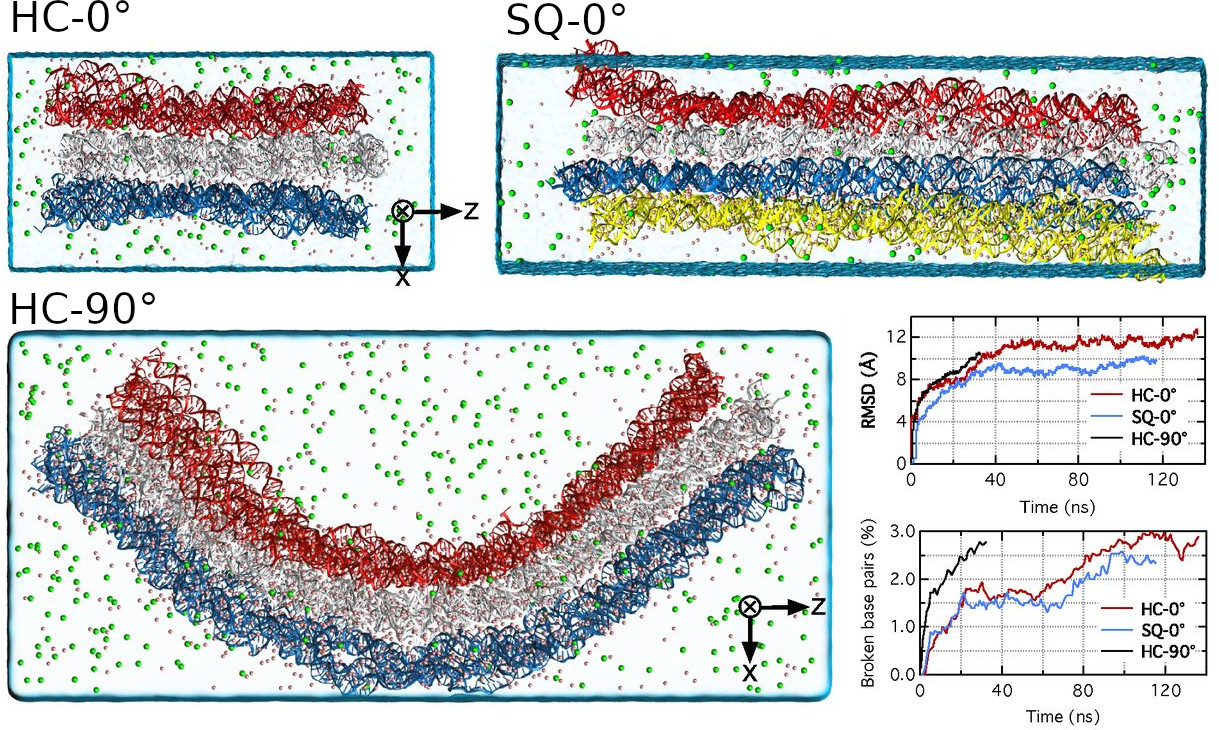
\includegraphics[width=\textwidth]{figures/all-atom.jpg}
    \caption{All-atom simulation of three DNA origami structures, adapted from \cite{yoo2013situ}. HC-0$^{\circ}$ is a honeycomb (hexagonal) lattice origami with no programmed curvature, while SQ-0$^{\circ}$ is designed on a square lattice. HC-0$^{\circ}$ has a programmed 90$^{\circ}$ bend. The plots show the root-mean-square deviation from the original atom positions (top) and the fraction of base pairs broken during the simulation (bottom).}
    \label{fig:all-atom}
  \end{center}
\end{figure}

\subsection{oxDNA/RNA}
\label{sec:oxDNA}
In 2010, a coarse-grained simulation software called oxDNA was introduced by Thomas Ouldridge \cite{ouldridge2010dna}. It runs molecular Dynamics (MD) and Monte Carlo (MC) simulations of DNA at the level of nucleotides and can model complex origami devices with a generally good agreement with experimental data \cite{sharma2017characterizing}.

Since its creation, both the model and the software running it has been extended and improved \cite{ouldridge2011structural, rovigatti2015comparison, sulc2012Sequence, ouldridge2013optimizing, snodin2015introducing}. In 2014, the model was extended to include RNA by Petr {\v{S}}ulc \cite{vsulc2014nucleotide}, showing its ability to model a set of common RNA motifs. In 2021, the model was further extended to include protein-DNA/RNA hybrids by Jonah Procyk \cite{procyk2021coarse}.


% OxDNA was joined by cogli1 for trajectory visualisation.


% Mention ANM model by Jonah!!!

While oxDNA can be very useful for modelling a structure, it has traditionally not been very accessible for experimentalists. Allthough efforts have been made create helpful tutorials \cite{doye2020oxdna}, users still needed an understanding of the command line to compile and run the code. This changed in 2020, with the launch of the \url{www.oxdna.org} web server \cite{oxdna.org}, where users can submit structures and setup and analyse simulations through a simple web interface.

\begin{figure}[h]
\begin{center}
    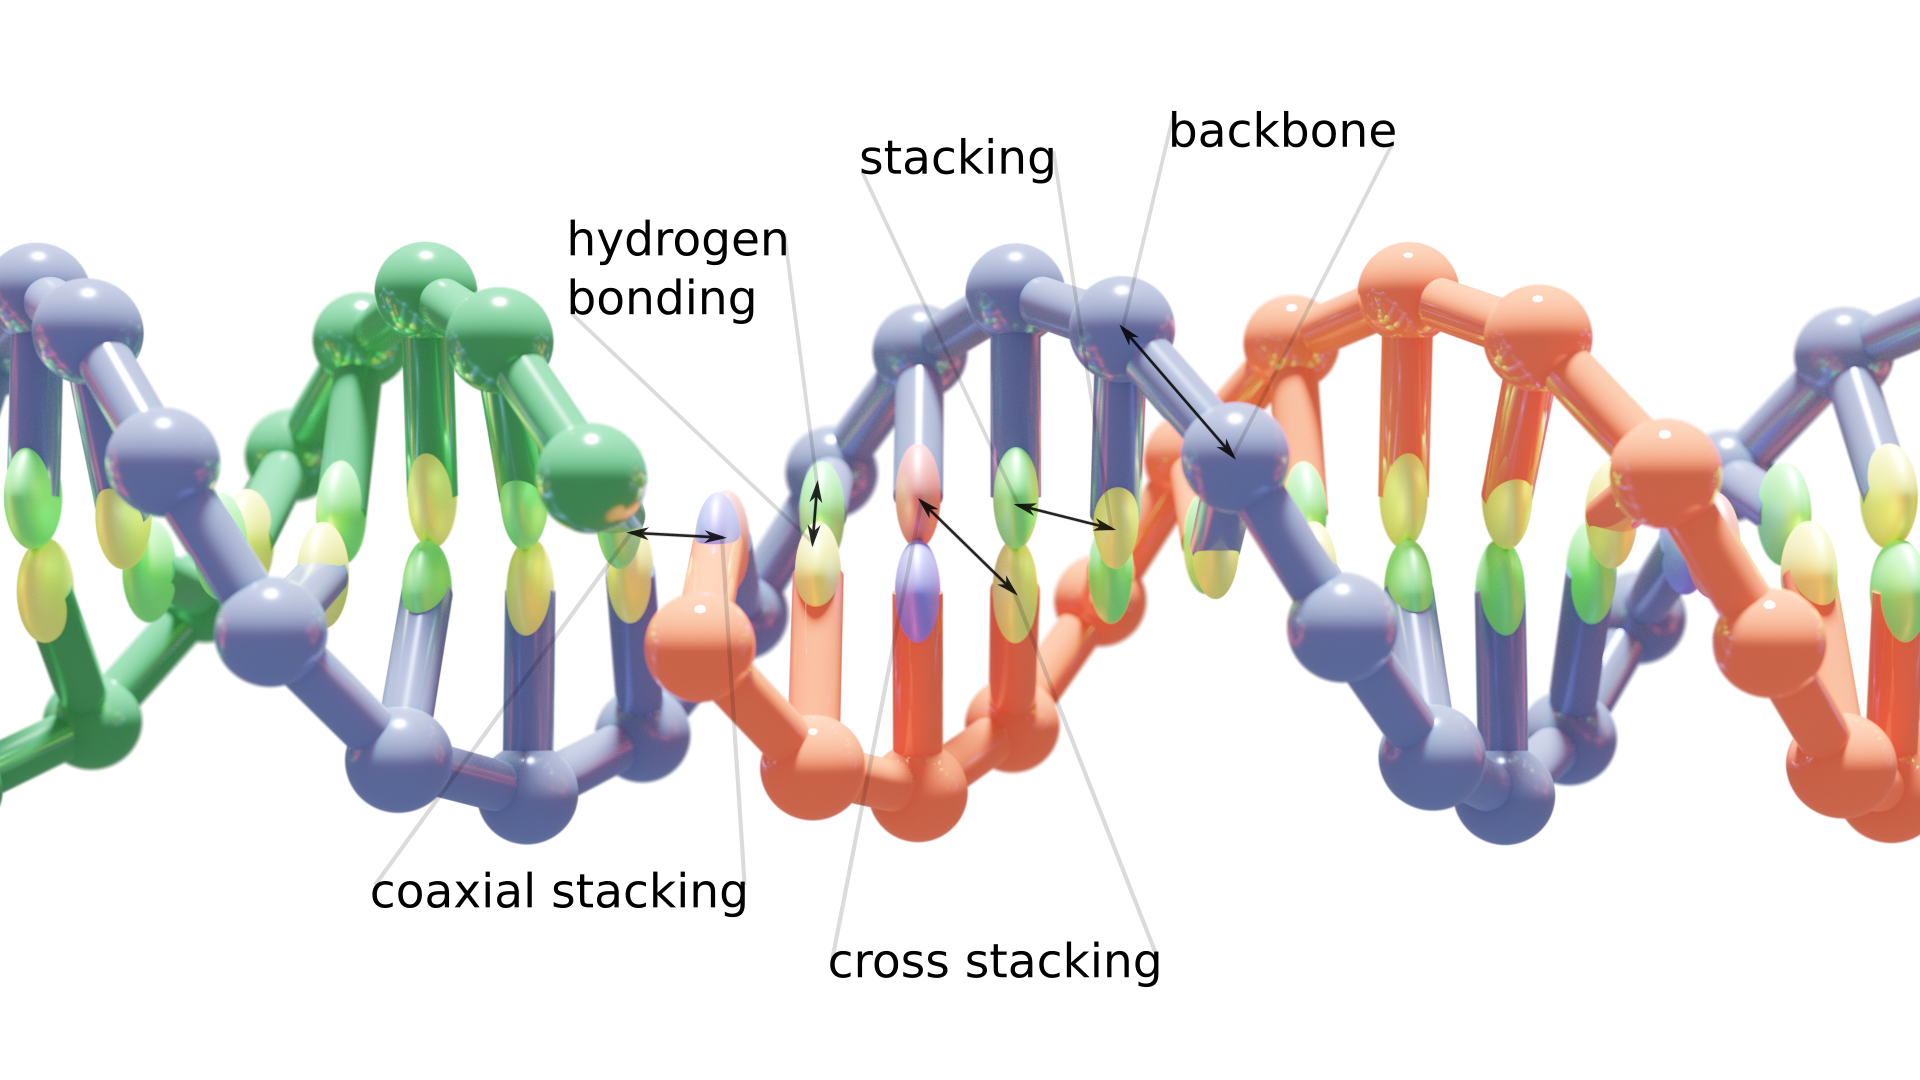
\includegraphics[width=\textwidth]{figures/oxdna_annot.png}
    \caption{The interaction forces of the oxDNA model. Each nucleotide is modelled as a rigid body with four interaction sites; a backbone repulsion site, a base repulsion site, a stacking site and a hydrogen bonding site. Apart from the five interactions annotated in the image, nucleotides also have an excluded volume, created through the two repulsion sites. The image was created in oxView and rendered in Blender}
    \label{fig_oxDNA}
    \end{center}
\end{figure}

\subsection{mrDNA}
\label{sec:mrdna}
The mrDNA simulation model \cite{maffeo2019mrdna} is a multi-resolution model representing a user-defined number of base pairs as a rigid-body bead.

Since mrDNA is implemented in Python and has a spline-based helix representation, users can write scripts to edit the structure, translating and rotating parts before starting the simulation. Thus, topological issues or over-stretched bonds can, with some skill, be resolved even before starting to simulate.

I did, based on this, also create a rudimentary interactive editor interface to mrdna, but it would need a lot of refinement to be externally usable. More importantly, the oxView editor, described in Chapter~\ref{ch:oxview}, can now easily resolve such issues.

\begin{figure}[h]
  \begin{center}
    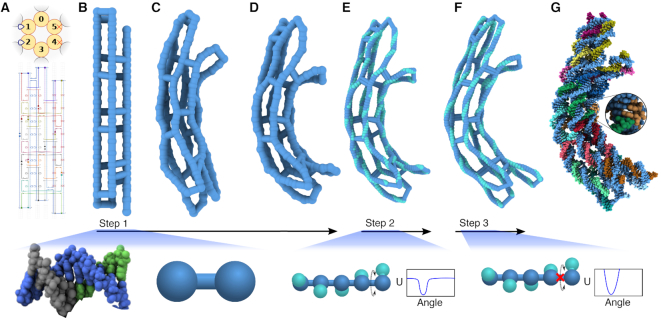
\includegraphics[width=\textwidth]{figures/mrDNA.jpg}
    \caption{MrDNA}
    \label{fig:mrdna}
  \end{center}
\end{figure}

A selection of the DNA designs I have relaxed are shown in Figure~\ref{fig:oxDNA_sims}. The first two examples, from \cite{gerling2015dynamic} and \cite{zadegan2012smallbox} and illustrated in Figure~\ref{fig:oxDNA_sims}.a) and~\ref{fig:oxDNA_sims}.b), are both quite straightforward to relax in oxDNA, although the relaxation is much faster using mrDNA.

The tensegrity kite structure, from \cite{liedl2010_kite} is harder to relax since, as seen in the first image in Figure~\ref{fig:oxDNA_sims}.c, the two helix bundles are drawn parallel to each other in caDNAno. Given enough time to relax, they should still become orthogonal, but a much more efficient way is to write a mrdna script to rotate one helix bundle so that it is orthogonal from the start, as seen in the middle image of~\ref{fig:oxDNA_sims}.c. The remaining overstretched bonds are then quickly relaxed using mrdna.

Finally, the Möbius strip, from \cite{han2010moebius}, is particularly tricky to relax, since the caDNAno design have all helices drawn in the same plane, with bonds from each end stretching through the whole structure and intersecting at a single point, as can be seen in the first image of Figure~\ref{fig:oxDNA_sims}.d. With some help from Chris Maffeo, however, I was able to use a mrdna script to edit the structure into a configuration much easier to relax, as seen in the second image of Figure~\ref{fig:oxDNA_sims}.d. Since the caDNAno design does not make it clear if the Möbius strip should be left-handed or right-handed, this is also decided in the script; changing the rotational direction will produce a mirrored version of the structure, as seen in the third image of Figure~\ref{fig:oxDNA_sims}.d.

\begin{figure}
  \centering
  \begin{overpic}[width=\textwidth]{figures/oxdna_sims.eps}
    \put(0,960){a)}
    \put(0,760){b)}
    \put(0,540){c)}
    \put(0,260){d)}
  \end{overpic}
  \caption{Relaxation results for various DNA designs. Each row depicts a new design, with the left-hand side showing the structure as it was drawn in caDNAno (and parsed by mrdna), while the right-hand side is the relaxed structure in oxDNA. Intermediate images are edits done in mrdna. While the switch design \cite{gerling2015dynamic} in  \textbf{a)} 
  and the small DNA origami box \cite{zadegan2012smallbox} in  \textbf{b)} relaxed without any required editing, the tensegrity kite structure \cite{liedl2010_kite} in  \textbf{c)} and the Möbius strip \cite{han2010moebius} in  \textbf{d)} benefited greatly from moving selected helices to a position off the lattice before starting the simulation.}
  \label{fig:mrdna}
\end{figure}

\subsection{Cando}

Cando is a finite element modelling framework \cite{castro2011primer, kim2012cando} available through a web server at \url{https://cando-dna-origami.org}. DNA double helices are modelled as elastic rods (connected by rigid crossovers) that stretch, twist and bend in line with experimental measurements. See Figure~\ref{fig:cando} for a set of example structures designed in caDNAno and simulated in Cando.

\begin{figure}[h]
  \begin{center}
    \begin{overpic}[width=\textwidth]{figures/cando.png}
      \put(0,670){a)}
      \put(500,670){b)}
      \put(0,300){c)}
      \put(810,300){d)}
    \end{overpic}
    \caption{Cando simulation results. Adapted from \cite{castro2011primer}. caDNAno design diagrams, Cando structure and flexibility prediction, and negative-stain TEM micrographs \textbf{a)} 90 degree gear. \textbf{b)} 180 degree gear. \textbf{c)} ``Robot'' design \textbf{d)} 60-helix bundle.}
    \label{fig:cando}
  \end{center}
\end{figure}